\documentclass{article}
\usepackage[margin=2cm]{geometry}
\usepackage{listings}
\usepackage{float}
\usepackage{graphicx}


\lstset{basicstyle=\footnotesize, columns=fullflexible}

\setlength{\parskip}{10pt plus 1pt minus 1pt
\setlength{\parindent}{0cm}}

\begin{document}
\title{CS26410 - Occupancy Grid Mapping Report}
\author{Samuel Jackson \\ \texttt{slj11@aber.ac.uk}}
\date{\today}
\maketitle


\section{Player and Stage}
The Player program together with the Stage plug-in provide a convenient controller and simulator pair for use in the field of robotics. Player acts as a wrapper to the hardware specifics of a robot and its sensors and provides an interface for an application to communicate with a physical robot. This is extremely useful, as it allows the developer to easily port code between different types and models of robots with different configurations and sensors without worrying too much about the underlying hardware. It also allows the developer to jump right into developing a robot controller, rather than dealing with code to interface with the system.

The Stage program is a plug-in for Player which is used to simulate a robot. Stage takes instructions from the Player application (which in turn is controlled by the developers code) and actuates a model of a robot within a simulated environment. In response, Stage also simulates sensor data relative to the position, speed, angle etc. of the robot and feeds it back into Player. This is useful as development of robot controllers can be made and testing without having access to a physical robot which can be both expensive and delicate. A simulation program such as Stage allows the core development of robot controllers on a smaller budget and without risk of damaging the robot through unforeseen bugs. The controllers can then be tested, tweaked and improved on a physical robot.

\section{Occupancy Grid Mapping}
Occupancy gird mapping is a robot mapping technique where the world is represented as a discrete number of equally sized, square chunks called cells. Each of these cells represents a position in a Cartesian coordinate system. Each of these cells can be labelled according to what a robot senses is at this position on the grid (such as if the cell is occupied by an object or not).

\subsection{Representing the world}
In my presented solution, I have split the world into a collection of cells which are 60x60 cm spanning from position (0,0) to an unspecified height and width using a 2D vector representation. Initially, only a grid of 6 x 6 cells are created, but as the robot explores the grid is able to dynamically resize to ensure that the robot never "falls off the map". 

Resizing the only occurs when a measured point if found to lay outside of the existing grid. When resizing in a negative direction, we must also shift all data elements forwards (or up) in order to keep the grid correctly positioned relative to the robot's position.

\begin{center}
	\begin{lstlisting}[language=c++, showstringspaces=false, caption={C++ code for dynamically resizing the grid when a point (x,y) falls outside the current grid's size}]

	if((x < 0 || y < 0) ||(x >= grid_width || y >= grid_height)) {
		
		x_expand = (x < 0 || x >= grid_width) ? EXPANSION_SIZE : 0;
		y_expand = (y < 0 || y >= grid_height) ? EXPANSION_SIZE : 0;

		new_width = grid_width + x_expand;
		new_height = grid_height + y_expand;

		//resize grid to new dimensions
		grid.resize(h);
		for (int i = 0; i < h; ++i) {
 			grid[i].resize(w);
 		}
		
		//if we did a negative resize, shift data
		if(x < 0 || y < 0) {
			robot_x += (x_expand*MAP_SCALE);
			robot_y += (y_expand*MAP_SCALE);

			x += EXPANSION_SIZE;
			y += EXPANSION_SIZE;

			for (int i = (grid_width-1); i >= 0; i--) {
				for (int j = (grid_height-1); j >= 0; j--) {
					int value = GetCell(i,j);
					SetCell(i+x_expand,j+y_expand,value);
					SetCell(i,j,0);
				}
			}
		}

		grid_width = new_width;
		grid_height = new_height;
	}
		
	\end{lstlisting}
\end{center}

Real world values for the robots change in position are fed into the mapping system and the robots position in the grid is updated relative to its position in the grid's coordinate system rather than Stage's coordinate system. This is because we require the index of each of cells to be positive so they can be applied to the 2D vector.

\subsection{Sensing the world}
As the Pioneer robot moves though the world (or the simulator) it can sample data from each of it's sensors and feed the data into the mapping system for evaluation. The sonar sensors used by the Pioneer robots can only give us information on the range (between 0-5 metres) of how far away something is relative to the position of the robot.

However, as we have access to the position of the robot, the angle it's facing and the distance to the sensed object, simple trigonometry can be used to estimate the likely location of the sensed point.

\[ x_{sensed} = x_{robot} + \cos (\theta) \times range \]
\[ y_{sensed} = y_{robot} + \sin (\theta) \times range \]

Where $x_{sensed}$ and $y_{sensed}$ are the position of the sensed point,$x_{robot}$ and $y_{robot}$ are the robot's current position, $\theta$ is the range of the sensor is currently pointing relative to 0 and range is the range the sensor measured too.

\begin{center}
	\begin{lstlisting}[language=c++, showstringspaces=false, caption={C++ code used for calculating the new point given the current position, angle and range}]

void OccupancyGrid::SensorUpdate(double range, double angle) {
	double sensor_x, sensor_y;

	if (range < MAX_RANGE) {

		//new point hit by sensor
		sensor_x = robot_x + (cos(angle) * range);
		sensor_y = robot_y + (sin(angle) * range);

		grid_x = ScaleToGrid(sensor_x);
		grid_y = ScaleToGrid(sensor_y);

		double max_grid_r = (MAX_RANGE/MAP_SCALE);
		double range_prob = (max_grid_r-range)/max_grid_r;

		SetCell(grid_x, grid_y, GetCell(grid_x, grid_y) + range_prob);
	}
}

	\end{lstlisting}
\end{center}

Once this new position has been obtained, we can scale and round it to the nearest cell in the grid and mark it as being occupied. In my controller, I am adding a value to the cell that represents the probability of the cell being occupied, which is inversely proportional to the range measured, as this cell is measured more and more and at closer ranges, the value increases proportionally to the certainty we have that the cell is occupied. Using this technique we can move through the world, make readings using the robot's sensors and build up a map of the world around us which could later be used for navigation.

In my example controller, I am simply using a random wander technique to move through the world and collect information about the system. This involves using simple reactive techniques to prevent the Pioneer from crashing into obstacles while still encouraging exploration of the environment. Below I provide a listing of the code I have used to get the robot moving around the simulated environment and avoiding collisions.

\begin{center}
	\begin{lstlisting}[language=c++, showstringspaces=false, caption={C++ code used to make control the robot to reactively wander through the environment}]

	for (;;) {
		robot.Read();

		//do simple collision avoidance
		if(sp[3] < 0.6 || sp[4] < 0.6) {
			int direction = (sp[3]<sp[4]) ? -1 : 1;
		} else if((sp[0] + sp[1]) < (sp[6] + sp[7])) {
			turnrate = dtor(-10);
		} else {
			turnrate = dtor(10);
		}

		if(sp[3] < 0.6 || sp[4] < 0.6) {
			speed = 0;
		} else {
			speed = 0.150;
		}

		//command the motors
		pp.SetSpeed(speed, turnrate);
	}

	\end{lstlisting}
\end{center}

The above system works by trying to keep the robot a balanced distance between the side a further front sensors. If the distance on one side becomes to large then it turns back towards the other direction. If the distance in front of the robot becomes too small then it reacts by turning on the spot until it has enough room to move off forward again. The robot will continue mapping in this way indefinitely. The following screen shot shows an example output from the terminal once mapping is complete:

\begin{figure}[H]
\centering
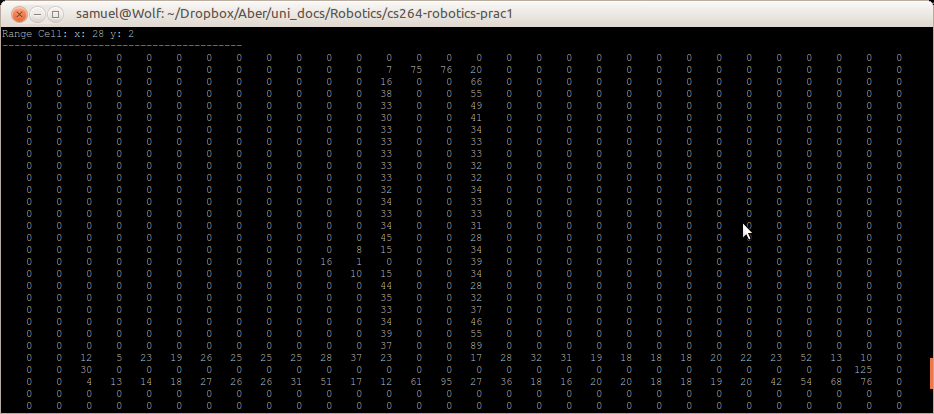
\includegraphics[width=1\textwidth]{example_run.png}
\caption{Console output from a typical simulation.}
\label{fig:example-run}
\end{figure}

\subsection{Interpreting Results}
Once we have mapped the environment, we can begin to analyse the quality of the map sensed and use a threshold to remove any values that appear to be incorrectly identified as walls and obstacles (more on why this occurs in section \ref{sec:issues})

One way of removing values from the map that have most likely been incorrectly identified as being occupied is to generate a threshold value. The threshold value acts as a cut off point. All values below the threshold are marked as being empty rather than occupied as they have most likely been misidentified. In my application, I have calculated the lower quartile of the data and used this as the threshold. This seemed a logical choice as it means any square above 25\% certainty will be classed as a wall. 

\begin{center}
	\begin{lstlisting}[language=c++, showstringspaces=false, caption={C++ code used to calculate the threshold value for the grid}]

void OccupancyGrid::CalculateThreshold() {
	using namespace std;
	double average = 0, lower_q = 0;
	vector<double> lq;
	vector<double> vec = VectorUtils::Flatten(grid);
	
	average = VectorUtils::Average(vec);
	vec = VectorUtils::Filter(vec, 0);
	for (int i = 0; i < vec.size(); i++) {
		if(vec[i] <= average) {
			lq.push_back(vec[i]);
		}
	}

	lower_q = VectorUtils::Average(lq);
	cout << "Threshold: " << lower_q+1 << endl;
}

	\end{lstlisting}
\end{center}

The following heat map shows analysis of a typical run of the map. The intensity of colour represents the certainty that the square is a wall. You can clearly see the comparison between the plain map (left) and the map with the threshold applied (right). While this method is by no means perfect, as you can see, it does help to remove some of the errors from grid and diminish the presence of others (more on this in section \ref{sec:issues}.
 
\begin{figure}[H]
\centering
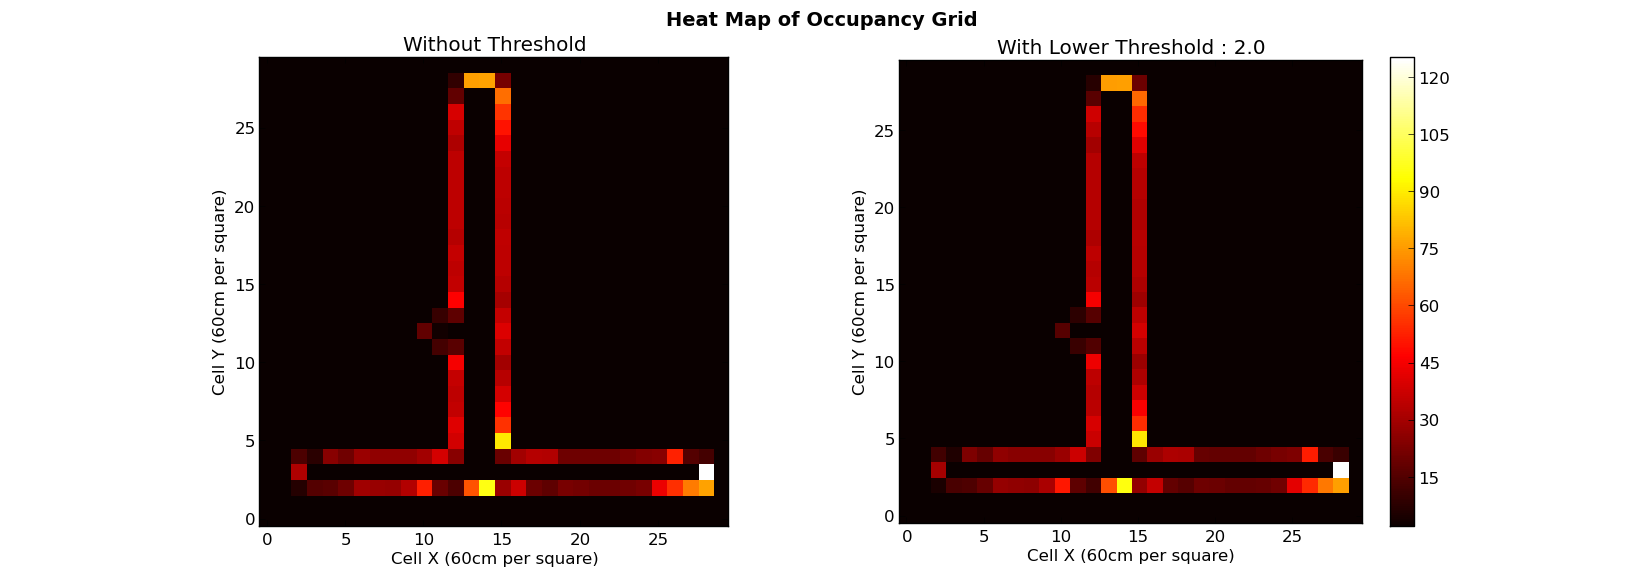
\includegraphics[width=1.1\textwidth]{final_example.png}
\caption{Heat Map showing the certainty that each cell in the grid is a wall. Left plot shows before the threshold is applied. Right plot shows after the threshold has been applied. Notice how the incorrect wall square in the nook is removed in the right hand plot.}
\label{fig:final-example}
\end{figure}

\subsection{Issues and Potential Improvements}
\label{sec:issues}
While I believe I have demonstrated a system that does a reasonable job of mapping and environment, I have encountered several areas of my application that could be vastly improved.

One issue that I have had with this problem is the inaccuracy of the sensors on the Pioneers and with sonar in general. When the Pioneer actively senses its environment, it sends a sonar pulse out from the sensor. This pulse spreads out at an angle of $15\,^\circ$. This means that the actual range measured will not necessarily be at the point exactly calculated from the robot's position, but could be anywhere within this $15\,^\circ$ field of view. Therefore at larger ranges, the accuracy of where the point is becomes less certain.

This problem is a major reason why points are incorrectly labelled as walls. Unfortunately, as the only information we are able to get from the sensor is the range it measured, there is no easy solution to this problem. However there are several ways that it can be diminished. 

One way is to limit the maximum range of a reading so that the ping produced does not get overly spread out. Another improvement is to only increment a cell by a value that is inversely proportional to the range of the measurement. This means that the value of the cell is directly proportional to the certainty we have about it being a wall. 

A final improvement that could be done in this area is the use of probability based on the contents of surrounding cells (i.e. if all neighbours are walls this cell is more likely to be a wall). However this approach would prove to be fairly complex and would require a lot more investigation beyond the scope of this report.

Another major issue that I have found using occupancy grid mapping is that the world (both simulated and real) can not always be split into a perfect grid. A wall or obstacle may intersect a cell only partially or at an awkward angle. This means that some space which is actually empty will be marked as being occupied. This problem could be potentially be solved by splitting each cell into a smaller collection of cells and analysing each one using the same technique as as before but on a smaller scale. This allows us to achieve a finer degree of accuracy for the reading, but at extra computational overhead.

Further improvements could also be made to the threshold value used in mapping. While the current value does a decent job of stripping out most of the incorrectly marked cells, it can be affected by outliers which have gained especially high or low readings during mapping, thus pulling up the threshold value. To combat this we can take into account a greater weighting of the values towards the smaller values in the dataset.

Alternatively we could use a clustering technique such as Otsu's method in order to find a decent threshold value to separate walls from empty space. However, this technique very much relies on a clear distinction between cells in both categories which may not necessarily be present in our collected data depending on how well we managed to measure them. Techniques such as this can also be affected if we map the same area more than once, thus raising the value stored in that position for the occupancy grid.

Finally, moving obstacle detection (i.e something that acts as a wall but can move or be removed) has not really been considered as part of this report. However I feel that my approach could be developed further to account for moving obstacles. Currently if the robot detects a obstacle the degree of occupancy of a cell is incremented. As more readings hit the obstacles then the degree of occupancy increase more and more and we become more certain that the obstacle exists. If the object disappears while still in range then the occupancy value does not get incremented and therefore, as other cells are marked, will slowly become a less prominent feature in the world until it eventually drops below the threshold entirely and is removed from the map.

\end{document}

